\chapter{Introduction}

These lecture notes grew out of STAT 946---Topics in Deep Learning Theory, taught at the University of Waterloo in Fall 2025. I taught the course from handwritten notes based on papers that I had read or written, including work that was then nearing completion. One motivation for preparing this document is a question I am often asked: what is a good place to start reading about deep learning theory? My aim is to offer a deliberately subjective guide to several directions in the field, with an emphasis on questions connected to my own research program.

The document began as a series of lecture notes scribed by dedicated students; many of the submissions far exceeded what I had expected from an ungraded task. GPT Pro and, later, Sol Ultra have been invaluable in combining and editing the scribed notes with the original papers and handwritten notes, substantially reducing the time required while improving the correctness and completeness of the resulting manuscript. Roughly one week of evening work produced a seemingly decent first draft, but very soon I realized the notes required much more careful editing and lots of time commitment. I should say I remain not completely happy with the current version, especially as the prose currently still reads quite AI-like in many places, although I'm pretty confident the mathematical content is correct and complete.

These lecture notes focus on \emph{scaling limits} of neural networks.\footnote{In this Nonstandard Analysis edition, all asymptotic scaling regimes are formulated directly at unlimited hyperfinite scale in Robinson's $\aleph_1$-saturated enlargement $(\hR, \hN)$, equipped with the ring of limited hyperreals $\Lim$, the maximal ideal of infinitesimals $\Inf$ ($\approx$), the multiplicative group of appreciable hyperreals $\App = \Lim \setminus \Inf$ ($\asymp$), the standard-part homomorphism $\st : \Lim \to \R$, and Loeb probability spaces $\Loeb$ \cite{robinson1966nonstandard,loeb1975conversion,anderson1976nonstandard,goldblatt1998lectures}. Mufan Li's exposition and narrative structure are preserved as closely as possible.} On the one hand, the mathematics of scaling limits is elegant and worth studying in its own right. On the other hand, many theorists, myself included, would like this work to have practical consequences. It is therefore worth motivating the selection of topics before turning to the technical details, including why some subjects that others may regard as foundational are not emphasized here.

\section{Motivation}

Modern deep learning is, in many ways, an empirical science: researchers propose a method, scale it up, and compare its performance on benchmarks. In recent years, increasing model, data, and compute scale has become a particularly reliable route to improved performance. As industrial research laboratories train increasingly large models, the gap between theory and practice continues to widen. Many mathematical obstacles make theoretical progress difficult, which raises a basic question:
\begin{quote}
\itshape What is the best way for theory to contribute to deep learning?
\end{quote}

\begin{figure}[t]
\centering
\begin{tikzpicture}[
    box/.style={draw, rounded corners=3pt, minimum height=1.05cm, minimum width=2.45cm, align=center, font=\small},
    arr/.style={-{Latex[length=2.4mm,width=1.7mm]}, semithick}
]
\node[box] (prop) at (0,0) {Propose\\method};
\node[box, minimum width=2.0cm, minimum height=0.72cm] (scale) at (3.6,0) {Scale up};
\node[box] (meas) at (7.3,0) {Measure\\+ compare};
\draw[arr] (prop) -- (scale);
\draw[arr] (scale) -- (meas);
\draw[arr] (meas.north) .. controls +(0,0.95) and +(0,0.95) .. (prop.north);
\end{tikzpicture}
\caption{A recurring pattern in deep learning research: new ideas are often validated (or rejected) only after large-scale training runs.}
\label{fig:1.1}
\end{figure}

It is instructive to examine empirical practice for clues; the cycle is summarized in Figure~\ref{fig:1.1}. First, the cycle of proposing a method, scaling it up, and measuring it on benchmarks has important limitations. In particular, benchmark comparisons do not always identify a uniformly better method. Conclusions can change with the architecture, data regime, tuning budget, or evaluation protocol, even when the empirical literature is extensive. When extensive experiments still do not yield a stable comparison, what can theory contribute?

Yet empirical practice also reveals a striking regularity. Across several deep learning tasks and over substantial measured ranges, test loss often decreases predictably as model size, dataset size, or training compute increases \cite{hestness2017deep}. These empirical relations are called \emph{scaling laws}: when the remaining resources are not limiting, test loss is often well approximated by a power law in the resource being varied \cite{kaplan2020scaling}. A power law appears approximately as a straight line on log--log axes, as illustrated in Figure~\ref{fig:1.2}.

\begin{figure}[t]
\centering
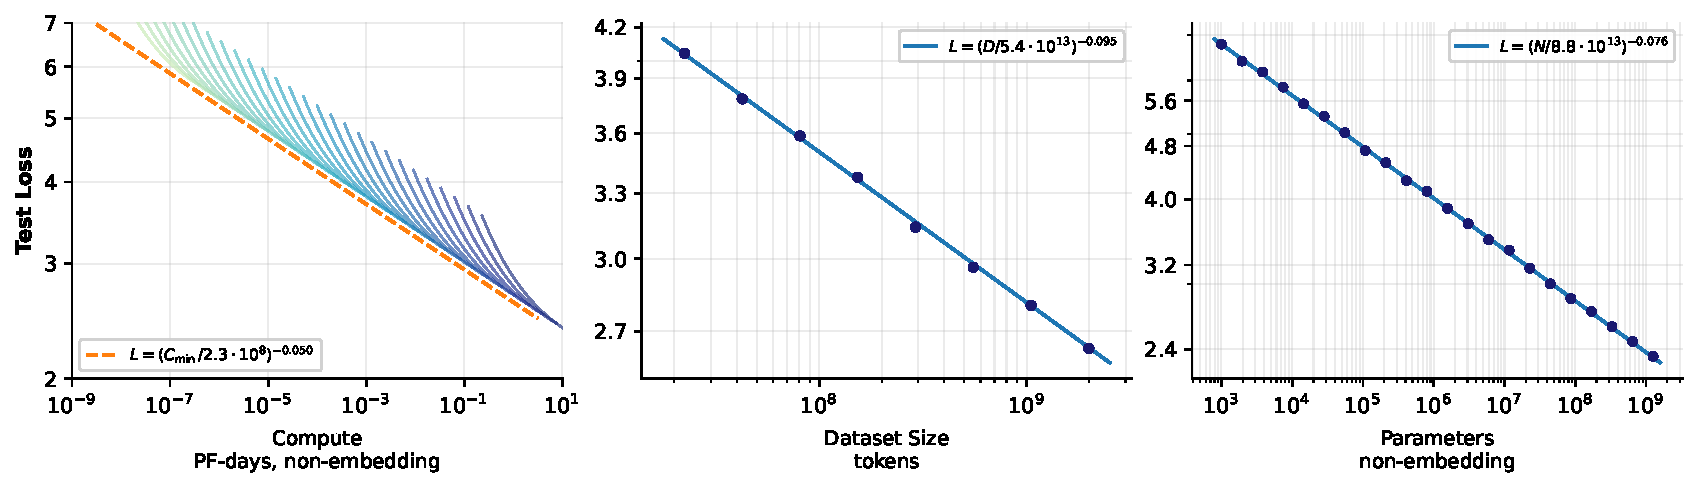
\includegraphics[width=\textwidth]{figures/fig1_2_scaling_laws.pdf}
\caption{Empirical neural-network scaling laws for language modeling (Kaplan et al.\ \cite{kaplan2020scaling}, Figure~1). On log--log axes, test loss decreases approximately as a power law in (left) training compute $C$, (middle) dataset size $D$, and (right) non-embedding parameter count $N$, within regimes not bottlenecked by the remaining resources.}
\label{fig:1.2}
\end{figure}

Within a fitted scaling regime, this predictability makes it possible to extrapolate larger-scale performance from smaller experiments \cite{kaplan2020scaling}. At a fixed training-compute budget, compute-optimal prescriptions jointly scale model size and training data rather than increasing either one in isolation \cite{kaplan2020scaling,hoffmann2022training}. The regimes of greatest practical interest, however, involve frontier models that can be prohibitively expensive to train. These observations raise two related questions: why should such simple power laws emerge from complex trained networks, and what can theory tell us about large models without paying their full computational cost?

One clue is that the same visual signature appears far beyond neural networks. Consider the log--log plot in Figure~\ref{fig:1.3}.

\begin{figure}[t]
\centering
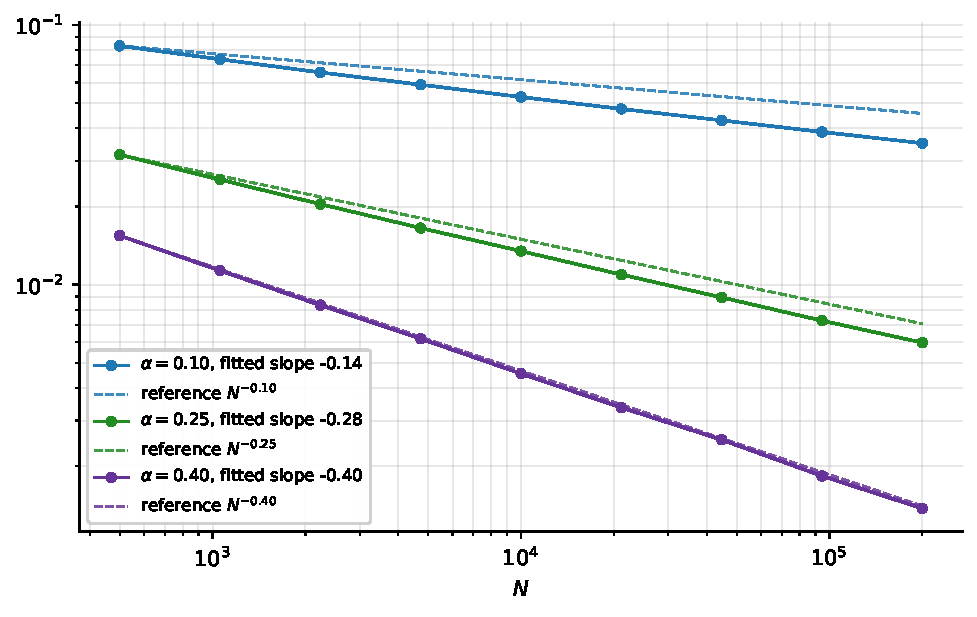
\includegraphics[width=0.72\textwidth]{figures/fig1_3_clt_rates.pdf}
\caption{A numerical central-limit-theorem convergence experiment. Solid curves show empirical Kolmogorov errors for three values of $\alpha$, while dashed lines show the corresponding $N^{-\alpha}$ reference rates.}
\label{fig:1.3}
\end{figure}

The resemblance is the point: this figure was not produced by training neural networks, but by simulating convergence toward the Gaussian limit for deliberately heavy-tailed summands. Related quantitative central limit theorems turn moment assumptions into power-law error bounds. For example, for i.i.d.\ centered, unit-variance summands, if $\E[\abs{X_1}^{2+2\alpha}] < \infty$ for some $\alpha \in (0, 1/2]$, then by transfer of a generalized Berry--Esseen bound \cite[Chapter~V]{petrov1975sums}, at any unlimited hypernatural $N \in \hNinf$ the internal Kolmogorov distance to ${}^*\Phi$ is bounded by $C N^{-\alpha} \in \Inf$ (infinitesimal of scale $N^{-\alpha}$). The broader point is that a straight line on log--log axes can record the infinitesimal scale at which a hyperfinite system approaches its standard shadow.

This comparison suggests viewing a neural-network scaling law as a finite-size (infinitesimal) correction to an underlying scaling limit. A scaling law describes how an observable changes with scale, whereas a scaling limit describes the standard shadow that the underlying hyperfinite system lies infinitely close to. Although trained neural networks of different sizes and architectures have different parameter spaces, we may nevertheless regard:
\begin{itemize}
\item $\mathcal{X}$ as a common space of trained neural networks for a fixed task and their possible scaling limits (with nonstandard extension ${}^*\mathcal{X}$). Unlike a predictor space, $\mathcal{X}$ may retain architecture- and parameter-level information while respecting hidden-unit permutation symmetries;
\item $x_N \in {}^*\mathcal{X}$ as the internal trained neural network obtained with unlimited hyperfinite compute budget $N \in \hNinf$, with the number of parameters, data points, and training iterations allowed to vary internally with $N$;
\item $L : \mathcal{X} \to \R$ as a test function, or observable, on this space, such as expected test loss (with natural extension ${}^*L : {}^*\mathcal{X} \to \hR$); and
\item $x_\infty \in \mathcal{X}$ as the standard shadow approached by $x_N$ ($x_N \approx x_\infty$ in ${}^*\mathcal{X}$), with $L_\infty := L(x_\infty) = \st({}^*L(x_N))$.
\end{itemize}
Suppose, heuristically, that $x_N \approx x_\infty$ in ${}^*\mathcal{X}$ and that ${}^*L$ detects the leading hyperfinite-compute correction nondegenerately. If this infinitesimal correction has scale $N^{-\alpha}$ for standard $\alpha > 0$, then
\begin{equation}\label{eq:1.1}
{}^*L(x_N) = L_\infty + c N^{-\alpha} + \varepsilon N^{-\alpha}, \qquad c \in \R \setminus \{0\}, \quad \varepsilon \approx 0,
\end{equation}
equivalently $\st\!\left(N^\alpha({}^*L(x_N) - L_\infty)\right) = c$ under an infinitesimal microscope of magnification $N^\alpha$. In this sense, the convergence rate seen through the test function $L$ appears by transfer at large standard scales as a scaling law. This conclusion is not automatic for every observable: regularity is needed, and cancellations or degeneracies can change the leading exponent. Because $N$ indexes compute, \eqref{eq:1.1} already has the familiar form of a loss--compute scaling law.

This is presently a research program rather than a derivation of the empirical loss laws observed in frontier models. Most available results vary only part of the system, for example width and depth while holding the dataset and training horizon fixed. Nevertheless, the classical example above makes the proposed mechanism plausible: when a quantitative scaling limit has an algebraic infinitesimal scale, suitable observables exhibit power-law finite-size corrections, and empirical neural-network scaling laws may reflect the same general mechanism.

This viewpoint is also particularly well suited to the current era of ever larger models. Frontier systems are increasingly expensive to study by direct experimentation and increasingly unwieldy to describe exactly at finite size. Scaling limits are designed for precisely this situation: they replace a growing family of complicated systems by a tractable standard shadow while retaining hyperfinite microscope information about how the finite systems approach that shadow. They therefore promise both a possible explanation of scaling laws and a practical language for reasoning about systems that cannot be studied exhaustively at their largest scale.

These considerations lead to two recurring goals:
\begin{enumerate}
\item use quantitative scaling relations to understand finite-scale behavior and determine when small networks are informative about larger networks; and
\item replace complicated finite networks by simpler limiting standard shadows.
\end{enumerate}

The success of hyperparameter transfer illustrates the first point: under a suitable parameterization, hyperparameters tuned on small networks can transfer to much larger ones \cite{yang2022tensor}. When the standard-part approximation is stable across the candidate hyperparameters, small networks can therefore serve as useful proxies for selecting hyperparameters in larger networks. In particular, the mechanisms supporting hyperparameter transfer need not be confined to a single scaling regime: Section~4.4 develops the $\mu$P width scaling, while Section~6.3 studies feature learning in a distinct proportional depth--width limit. The following examples emphasize the second point by showing how nonstandard scaling limits replace complicated hyperfinite systems with simpler standard objects; hyperfinite expansions additionally describe how the finite systems approach those shadows.

\section{Examples of Scaling Limits}

We now return to the Central Limit Theorem (CLT), whose quantitative form supplied the motivating plot in Figure~\ref{fig:1.3}. Its qualitative statement already has the structure of a scaling limit: normalized hyperfinite sums of internal i.i.d.\ summands project under the standard-part map to a simple, universal Gaussian law. Fix $N \in \hNinf$, and let $(X_i)_{i=1}^N$ be an internal i.i.d.\ sequence on an internal probability space $(\Omega, \mathcal{A}, \hP)$ with $\hE[X_i] = 0$, $\hVar(X_i) = \sigma^2 \in (0,\infty)$, and S-integrable squares. Equipped with the Loeb probability measure $\Loeb$ \cite{loeb1975conversion,cutland2000loeb}, the hyperfinite CLT states that $S_N := \frac{1}{\sigma\sqrt{N}}\sum_{i=1}^N X_i \in \Lim$ $\Loeb$-almost surely and
\begin{equation}\label{eq:1.2}
\st\!\left(\frac{1}{\sigma\sqrt{N}}\sum_{i=1}^N X_i\right) \sim \mathcal{N}(0, 1) \qquad \text{under } \Loeb.
\end{equation}
The remarkable aspect is universality: only the first two moments matter for the standard shadow. The scaling $1/\sqrt{N}$ is not cosmetic: it simultaneously keeps the internal variance in $\App$ (appreciable, order one) and ensures each individual term contributes an infinitesimal of scale $1/\sqrt{N} \in \Inf$. Quantitative versions of the CLT additionally control the infinitesimal distance between the internal distribution and ${}^*\mathcal{N}(0,1)$; Figure~\ref{fig:1.3} illustrates the power-law rates discussed above.

The CLT has a functional analogue: an internal rescaled hyperfinite random walk has standard Brownian motion as its uniform shadow \cite{anderson1976nonstandard}. Let $(X_i)_{i=1}^{\lceil NT\rceil + 1}$ be internal i.i.d.\ hyperreal random variables with $\hE[X_i] = 0$, $\hVar(X_i) = \sigma^2 \in (0,\infty)$, and S-integrable $X_i^2$. Define the internal normalized partial sums
\begin{equation}\label{eq:1.3}
Y_k^{(N)} := \frac{1}{\sigma\sqrt{N}}\sum_{i=1}^k X_i, \qquad k = 0, 1, \dots, \lceil NT\rceil + 1.
\end{equation}
To obtain an internal continuous path, linearly interpolate between consecutive hyperfinite steps:
\begin{equation}\label{eq:1.4}
Z_t^{(N)} := Y_{\lfloor Nt\rfloor}^{(N)} + (Nt - \lfloor Nt\rfloor)\!\left(Y_{\lfloor Nt\rfloor+1}^{(N)} - Y_{\lfloor Nt\rfloor}^{(N)}\right), \qquad t \in {}^*[0, T].
\end{equation}
For each fixed standard $t \in [0,T]$, the hyperfinite CLT implies $\st(Z_t^{(N)}) \sim \mathcal{N}(0, t)$ under $\Loeb$.

\begin{definition}[Brownian Motion]\label{def:1.1}
A stochastic process $(B_t)_{t\in[0,T]}$ is a (standard) Brownian motion if:
\begin{enumerate}
\item $B_0 = 0$ almost surely;
\item for $0 \le s \le t$, the increment $B_t - B_s \sim \mathcal{N}(0, t-s)$ and disjoint increments are independent;
\item $t \mapsto B_t$ is almost surely continuous.
\end{enumerate}
\end{definition}

For an internal random element $Z^{(N)}$ taking values in ${}^*\mathcal{X}$ for a Polish metric space $(\mathcal{X}, d)$ and a standard random element $Z$ in $\mathcal{X}$, $Z^{(N)}$ has Loeb shadow law $Z$ when $\st(Z^{(N)})$ exists $\Loeb$-almost surely and $\EL[{}^*\psi(Z^{(N)})] = \st(\hE[{}^*\psi(Z^{(N)})]) = \E[\psi(Z)]$ for every bounded continuous $\psi : \mathcal{X} \to \R$. Thus Loeb pushforward via $\st$ applies directly to hyperfinite random paths once their function space and metric are specified.

\begin{theorem}[Anderson's Hyperfinite Brownian Motion / Donsker's Invariance Principle \cite{donsker1951invariance,anderson1976nonstandard}]\label{thm:1.2}
Under the assumptions above, for $N \in \hNinf$, the internal path $(Z_t^{(N)})_{t\in{}^*[0,T]}$ is $\Loeb$-almost surely nearstandard (equivalently, limited and S-continuous: $s \approx t \implies Z_s^{(N)} \approx Z_t^{(N)}$) in ${}^*C([0,T])$ equipped with the internal sup norm, and its standard part $B_t := \st(Z_{\ns{t}}^{(N)})$ is a standard Brownian motion on $(\Omega, \mathcal{L}(\mathcal{A}), \Loeb)$ satisfying
\begin{equation}\label{eq:1.5}
\sup_{t \in {}^*[0, T]} \abs{Z_t^{(N)} - {}^*B_t} \approx 0 \qquad \Loeb\text{-almost surely}, \qquad \st(Z^{(N)}) \sim B \text{ in } (C([0,T]), \norm{\cdot}_\infty).
\end{equation}
\end{theorem}

\begin{remark}\label{rem:1.3}
This is the prototype for a hyperfinite diffusion approximation \cite{keisler1984infinitesimal,lindstrom1988invitation}: after identifying the correct infinitesimal local drift, diffusion variance, and hyperfinite step size $\Delta\tau = 1/N \in \Inf_+$, an internal discrete recursion projects via $\st$ to an It\^o SDE. The same template reappears in the depth-scaling arguments of Chapter~5 and is formalized in Appendix~A.3.
\end{remark}

A different type of scaling limit appears in random matrix theory, where a hyperfinite-dimensional internal random matrix has a deterministic standard spectral distribution. For $N \in \hNinf$, let $X \in \hR^{N\times N}$ be an internal symmetric matrix, with the entries on and above the diagonal internally independent and identically distributed, centered, of variance one, and with limited fourth moment. Consider the scaled matrix $N^{-1/2}X$, with internal real eigenvalues $\lambda_1^{(N)} \le \dots \le \lambda_N^{(N)}$. Define the internal \emph{empirical spectral distribution} (ESD)
\begin{equation}\label{eq:1.6}
\rho^{(N)}(dx) := \frac{1}{N}\sum_{i=1}^N \delta_{\lambda_i^{(N)}}(dx).
\end{equation}

\begin{theorem}[Wigner Semicircle Law \cite{wigner1958distribution}]\label{thm:1.4}
For $N \in \hNinf$, $\Loeb$-almost surely, the Loeb standard-part pushforward $\rho_{\mathrm{sc}} := L(\rho^{(N)}) \circ \st^{-1}$ is the deterministic probability measure (meaning $\int_{\hR} {}^*\psi(x)\,\rho^{(N)}(dx) \approx \int_\R \psi(x)\,\rho_{\mathrm{sc}}(dx)$ for every bounded continuous $\psi : \R \to \R$) with density
\begin{equation}\label{eq:1.7}
\rho_{\mathrm{sc}}(x) = \frac{\sqrt{(4 - x^2)_+}}{2\pi}, \qquad \text{supported on } [-2, 2].
\end{equation}
\end{theorem}

\begin{remark}\label{rem:1.5}
The emergence of a deterministic standard shadow spectrum is an example of self-averaging: macroscopic hyperfinite averages concentrate within a single monad at unlimited dimension $N \in \hNinf$. In the random-projection model of Chapter~3, standard-part spectra of hyperfinite design and Gram matrices determine explicit risk formulas.
\end{remark}

The final example replaces a hyperfinite interacting particle system by a deterministic evolution of its Loeb empirical shadow. Let $\mathcal{K} : \R \to \R$ be a bounded Lipschitz interaction kernel with natural extension ${}^*\mathcal{K} : \hR \to \hR$. Consider $N \in \hNinf$ internal particles $(X_i(t))_{i=1}^N$ in $\hR$ evolving according to the internal mean-field ODE system
\begin{equation}\label{eq:1.8}
\partial_t X_i(t) = \frac{1}{N}\sum_{j=1}^N {}^*\mathcal{K}\!\left(X_i(t) - X_j(t)\right).
\end{equation}
Define the internal empirical measure
\begin{equation}\label{eq:1.9}
\rho_t^{(N)}(dx) := \frac{1}{N}\sum_{i=1}^N \delta_{X_i(t)}(dx).
\end{equation}
For a probability measure $\rho$ on $\R$, define the law-dependent velocity field
\begin{equation}\label{eq:1.10}
b(x, \rho) := \int_\R \mathcal{K}(x - y)\,\rho(dy).
\end{equation}
Then the internal particle equation can be written exactly as $\partial_t X_i(t) = {}^*b(X_i(t), \rho_t^{(N)})$. With internal i.i.d.\ initial conditions of law ${}^*\rho_0$, $\Loeb$-almost surely the Loeb shadow measure $\rho_t := L(\rho_t^{(N)}) \circ \st^{-1}$ is the deterministic evolution $(\rho_t)$ governed by
\begin{equation}\label{eq:1.11}
\partial_t \rho_t + \partial_x\!\left(b(\cdot, \rho_t)\rho_t\right) = 0, \qquad \rho_{t=0} = \rho_0.
\end{equation}
The equation is interpreted in the weak sense; see Appendix~A.1.

Although the particles interact at hyperfinite $N$, the independence present at initialization survives in the standard-part shadow: for any fixed standard $k \in \N$, $(\st(X_1(t)), \dots, \st(X_k(t)))$ are independent samples from $\rho_t$ under $\Loeb$. This phenomenon is called \emph{propagation of chaos} \cite{sznitman1991topics}. Quantitative versions show that hyperfinite errors for suitable observables lie in $O(N^{-\alpha}) \subset \Inf$; a leading infinitesimal correction of scale $N^{-\alpha}$ corresponds by transfer to a scaling law for the approach to the mean-field shadow.

In mean-field analyses of neural networks, neurons or parameters play the role of hyperfinite particles. Their internal empirical distribution evolves under training and, at hyperfinite width $N \in \hNinf$, its Loeb shadow is described by a McKean--Vlasov transport equation of this type. We return to this connection in Chapter~4.

\begin{remark}[A Checklist for Scaling Limits]\label{rem:1.6}
The three examples have the same four nonstandard ingredients:
\begin{enumerate}
\item an internal hyperfinite random object at unlimited scale $N \in \hNinf$;
\item a normalization placing observables in $\Lim$ or $\App$ and a declaration of what is unlimited ($\in \hNinf$) and what remains standard;
\item nearstandardness (or S-continuity) in the target space under Loeb probability $\Loeb$; and
\item a standard shadow via $\st$ with a tractable description.
\end{enumerate}
For the random walk the shadow is a continuous path, for the Wigner matrix it is a probability measure, and for the particle system it is a deterministic evolution of probability measures. Later chapters repeat this template with network outputs, kernels, parameter distributions, and covariance processes. A quantitative scaling limit adds a further ingredient: an infinitesimal microscope magnification $N^\alpha$ isolating the leading hyperfinite correction for the observable of interest.
\end{remark}

\section{Roadmap}

The remainder of the lecture notes is organized as follows.

\textbf{Chapter~2} treats two related but logically distinct hyperfinite-width limits ($N \in \hNinf$) for wide fully-connected networks. At random initialization, the standard parts of the outputs on any fixed standard finite collection of inputs follow a centered Gaussian vector law under $\Loeb$ characterized by the neural network Gaussian process (NNGP) kernel. During gradient-flow training in the NTK, or lazy-training, regime, the internal tangent kernel at each standard training time lies infinitely close ($\approxP$) to a deterministic standard kernel $K$ that does not depend on time, reducing the standard-part output dynamics to kernel gradient flow.

\textbf{Chapter~3} turns from fitting the training data to prediction on new data. Using linear regression with hyperfinite random projections, it explains why test error can spike into the unlimited range ($\hR \setminus \Lim$) when the model first becomes able to fit the training data exactly and then decrease across appreciable values as more features are added.

\textbf{Chapter~4} introduces \emph{feature-learning} scalings in which internal representations evolve by an appreciable ($\in \App$) amount during training at hyperfinite width $N \in \hNinf$, including shallow mean-field limits via Loeb empirical measures, the maximal-update ($\mu$P) parameterization, and a sketch of DMFT for deep networks.

\textbf{Chapter~5} studies hyperfinite depth scalings ($D \in \hNinf$) and joint depth--width limits at initialization, including proportional hyperfinite limits $\st(D/N) = \bar{\tau} \in (0,\infty)$ and the neural covariance SDE viewpoint via Keisler--Lindstr\o m hyperfinite stochastic difference equations.

\textbf{Chapter~6} discusses several applications of the depth scaling theory, including shaped attention/transformer models, the limiting spectrum of the feature covariance, and a one-step feature-learning mechanism in the proportional hyperfinite limit.

Across these chapters, the principal regimes differ in what remains standard and what is taken unlimited in $\hNinf$:
\begin{itemize}
\item in Chapter~2, width $N \in \hNinf$ while depth $d$, input dimension $n_0$, and dataset size $m$ remain standard;
\item in Chapter~3, $(M, N_0, N) \in (\hNinf)^3$ are proportionally unlimited, with $\st(N_0/M) = \gamma \in (0,\infty)$ and $\st(N/M) = \delta \in (0,\infty)$;
\item in Chapter~4, width $N \in \hNinf$ under feature-learning parameterizations ($\gamma_N \asymp \sqrt{N}$) and associated learning-rate scalings ($\eta_N \asymp N$), including both the shallow mean-field and deep maximal-update ($\mu$P) regimes; and
\item in Chapters~5 and~6, depth $D \in \hNinf$ and width $N \in \hNinf$ can be jointly unlimited with $\st(D/N) = \bar{\tau}$, typically with a fixed standard collection of inputs before an additional hyperfinite spectral limit $M \in \hNinf$ is taken.
\end{itemize}

The technical appendix collects the Loeb weak-shadow, S-equicontinuity, Skorohod lifting, affine-invariant metric, and internal Gaussian-conditioning tools used across these regimes.
